\documentclass{article}
\usepackage{listings}
\usepackage{graphicx}
\graphicspath{ {./} }

\begin{document}
\title{CMOR 420\slash520, Homework \#4: \LaTeX\ Submission}
\author{\texttt{bi3}}
\date{December 8, 2023}
\maketitle

\section*{Verification}

\subsection*{Type stability}

\begin{verbatim}

julia> @code_warntype mul!(out, A_sparse, x)
MethodInstance for LinearAlgebra.mul!(::Vector{Float64},
  ::SparseMatrixCSR{Float64}, ::Vector{Float64})
  from mul!(out, A::SparseMatrixCSR, x::AbstractVector) @
  Main c:\Users\bciro\Desktop\cmor-420-520-f23-main\HW4\main.jl:52
Arguments
  #self#::Core.Const(LinearAlgebra.mul!)
  out::Vector{Float64}
  A::SparseMatrixCSR{Float64}
  x::Vector{Float64}
Locals
  @_5::Union{Nothing, Tuple{Int64, Int64}}
  @_6::Int64
  m::Int64
  @_8::Union{Nothing, Tuple{Int64, Int64}}
  i::Int64
  sum::Float64
  row_end::Int64
  row_start::Int64
  j::Int64
  col::Int64
Body::Nothing
1   %1  = Main.size(A)::Tuple{Int64, Int64}
    %2  = Base.indexed_iterate(%1, 1)::Core.PartialStruct(Tuple{Int64, Int64},
          Any[Int64, Core.Const(2)])
          (m = Core.getfield(%2, 1))
          (@_6 = Core.getfield(%2, 2))
    %5  = Base.indexed_iterate(%1, 2, @_6::Core.Const(2))::Core.PartialStruct(
          Tuple{Int64, Int64}, Any[Int64, Core.Const(3)])
          Core.getfield(%5, 1)
    %7  = (1:m)::Core.PartialStruct(UnitRange{Int64}, Any[Core.Const(1), Int64])
          (@_5 = Base.iterate(%7))
    %9  = (@_5 === nothing)::Bool
    %10 = Base.not_int(%9)::Bool
          goto #7 if not %10
2   %12 = @_5::Tuple{Int64, Int64}
         (i = Core.getfield(%12, 1))
    %14 = Core.getfield(%12, 2)::Int64
    %15 = Base.getproperty(A, :row_ptr)::Vector{Int64}
         (row_start = Base.getindex(%15, i))
    %17 = Base.getproperty(A, :row_ptr)::Vector{Int64}
    %18 = (i + 1)::Int64
         (row_end = Base.getindex(%17, %18))
         (sum = 0.0)
    %21 = row_start::Int64
    %22 = (row_end - 1)::Int64
    %23 = (%21:%22)::UnitRange{Int64}
         (@_8 = Base.iterate(%23))
    %25 = (@_8 === nothing)::Bool
    %26 = Base.not_int(%25)::Bool
          goto #5 if not %26
3   %28 = @_8::Tuple{Int64, Int64}
         (j = Core.getfield(%28, 1))
    %30 = Core.getfield(%28, 2)::Int64
    %31 = Base.getproperty(A, :col_indices)::Vector{Int64}
         (col = Base.getindex(%31, j))
    %33 = sum::Float64
    %34 = Main.getindex(A, i, col)::Float64
    %35 = Base.getindex(x, col)::Float64
    %36 = (%34 * %35)::Float64
         (sum = %33 + %36)
         (@_8 = Base.iterate(%23, %30))
    %39 = (@_8 === nothing)::Bool
    %40 = Base.not_int(%39)::Bool
          goto #5 if not %40
4         goto #3
5         Base.setindex!(out, sum, i)
         (@_5 = Base.iterate(%7, %14))
    %45 = (@_5 === nothing)::Bool
    %46 = Base.not_int(%45)::Bool
          goto #7 if not %46
6         goto #2
7         return nothing


julia> @code_warntype iterate(A_sparse, b, u, a)
MethodInstance for iterate(::SparseMatrixCSR{Float64}, ::Vector{Float64},
  ::Vector{Float64}, ::Float64)
  from iterate(A, b, u, a; tol) @ Main c:\Users\bciro\Desktop\
  cmor-420-520-f23-main\HW4\HW4.jl:145
Arguments
  #self#::Core.Const(iterate)
  A::SparseMatrixCSR{Float64}
  b::Vector{Float64}
  u::Vector{Float64}
  a::Float64
Body::Tuple{Vector{Float64}, Int64, Float64}
1   %1 = Main.:(var"#iterate#7")(0.001, #self#, A, b, u, a)
    ::Tuple{Vector{Float64}, Int64, Float64}
         return %1


julia> @code_warntype iterate(A_dense, b, u, a)
MethodInstance for iterate(::Matrix{Float64}, ::Vector{Float64},
  ::Vector{Float64}, ::Float64)
  from iterate(A, b, u, a; tol) @ Main c:\Users\bciro\Desktop\
  cmor-420-520-f23-main\HW4\HW4.jl:145
Arguments
  #self#::Core.Const(iterate)
  A::Matrix{Float64}
  b::Vector{Float64}
  u::Vector{Float64}
  a::Float64
Body::Tuple{Vector{Float64}, Int64, Float64}
1   %1 = Main.:(var"#iterate#7")(0.001, #self#, A, b, u, a)::Tuple{
    Vector{Float64}, Int64, Float64}
         return %1

\end{verbatim}

\section*{Timings}

\begin{verbatim}

julia> @time iterate(A_sparse, b, u, a)
  0.062693 seconds (55.07 k allocations: 47.019 MiB, 26.83% gc time)


julia> @time iterate(A_dense, b, u, a)
  1.217082 seconds (175.59 k allocations: 55.330 MiB, 0.81% gc time,
  8.68% compilation time)


\end{verbatim}

\section*{Plot of Initial/Final Solutions}

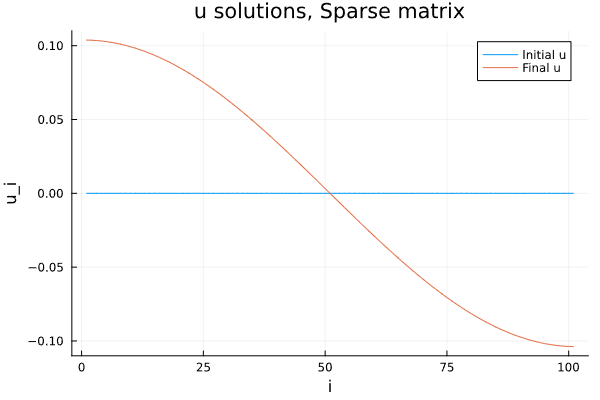
\includegraphics{SparseSolutions}

\section*{Different solvers}

When we solve for the ODE using Heun's method, we find that there are 39,957 function evaluations, with 19975 accepted steps and 3 rejected steps. In this case, the number of function evaluations is roughly double that of the number of accepted steps. If RK4 is used, less time steps are used (14350), but six times as many function evaluations (86101) as time steps are required. Finally, using BS3 required 47716 function evaluations with 15903 time steps; for this method, 2 steps were rejected. 

\section*{Errors}

There is one 'error' with my code. When I implemented rhs! and solved the system as the following:

\begin{verbatim}

function rhs!(du, u, p, t)
    du = p[1] - p[2] * u
end
interval = (0., 1.)
u0 = zeros(m+1)
prob = ODEProblem(rhs!, u0, interval, p)
sol1 = solve(prob, Heun(), dt = 0.5*h^2)

\end{verbatim}

The code would run, but my solutions were all vectors of zeros. When I replace rhs! with the following:

\begin{verbatim}

rhs(u, p, t) = p[1] - p[2]*u
interval = (0., 1.)
u0 = zeros(m+1)
prob = ODEProblem(rhs, u0, interval, p)
sol1 = solve(prob, Heun(), dt = 0.5*h^2)

\end{verbatim}

The above code runs and gives me the actual solutions. I don't know why this happens, but I implement the rhs version when solving the system, and will have commented code containing the rhs! version at the bottom of the file, in case you want to try running it yourself. 

\end{document}
